\documentclass{article}
\usepackage{amsmath}
\usepackage{listings}
\usepackage{xcolor}
\usepackage{graphicx}


\title{202A: Dynamic Programming and Applications\\[5pt] {\Large \textbf{Coding Homework \#2}}}

\author{Rafael Pintro Schmitt}

\date{}


\begin{document}

\maketitle 

\subsection*{Question 1}

1. Consumption Euler Equation at Steady State
\[
0 = \frac{\dot{c}}{c} = \frac{f'(k^*) - \rho - \theta g}{\theta}
\]
Given $\theta = 1$ and $f(k) = Ak^\alpha$ with $A = 1$, the equation simplifies to:
\[
f'(k^*) = \rho + g
\]
\[
\alpha k^{*\alpha - 1} = \rho + g
\]
\[
k^{*\alpha - 1} = \frac{\rho + g}{\alpha}
\]
Substituting $\alpha = \frac{1}{3}$, $\rho = 0.03$, and $g = 0.02$:
\[
k^{*-2/3} = \frac{0.05}{1/3} = 0.15
\]
\[
k^* = \left(6.\overline{6}\right)^{\frac{3}{2}} \approx 17.2136
\]
2. Capital Accumulation Equation at Steady State
\[
0 = f(k^*) - c^* - (n + g)k^*
\]
Solving for $c^*$:
\[
c^* = f(k^*) - (n + g)k^*
\]
\[
f(k^*) = k^{*\alpha} = 17.2136^{1/3} \approx 2.582
\]
\[
(n + g)k^* = 0.04 \times 17.2136 \approx 0.6885
\]
\[
c^* = 2.582 - 0.6885 \approx 1.8935
\]

\subsection*{Question 2}
\lstset{
    language=Matlab,
    basicstyle=\ttfamily\small,
    keywordstyle=\color{blue},
    commentstyle=\color{green!50!black},
    stringstyle=\color{red},
    numbers=left,
    numberstyle=\tiny,
    stepnumber=1,
    numbersep=5pt,
    backgroundcolor=\color{white},
    tabsize=4,
    showspaces=false,
    showstringspaces=false,
    breaklines=true,
    breakatwhitespace=true,
    frame=single,
    captionpos=b
}

\begin{lstlisting}
% MATLAB code to solve for the steady-state values of capital and consumption using fsolve

% Parameters
rho = 0.03;       % Discount rate
theta = 1;        % Inverse of intertemporal elasticity of substitution
g = 0.02;         % Technology growth rate
n = 0.02;         % Population growth rate
alpha = 1/3;      % Capital share
A = 1;            % Total Factor Productivity

% Steady-state equation for capital
steady_state_eq = @(k) alpha * A * k^(alpha - 1) - (rho + g);

% Initial guess for k*
k0 = 30;

% Solve for k* using fsolve
options = optimoptions('fsolve', 'Display', 'off');
[k_star, ~, exitflag] = fsolve(steady_state_eq, k0, options);

% Check if fsolve converged
if exitflag > 0
    % Compute steady-state consumption c*
    c_star = A * k_star^alpha - (n + g) * k_star;

    % Display the steady-state values
    fprintf('Steady-state capital per effective worker (k*): %.4f\n', k_star);
    fprintf('Steady-state consumption per effective worker (c*): %.4f\n', c_star);
else
    disp('fsolve did not converge to a solution.');
end
\end{lstlisting}
After which we get: Steady-state capital per effective worker (k*): 17.2039\\
Steady-state consumption per effective worker (c*): 1.8934\\

\subsection*{Question 3}

\begin{lstlisting}
% MATLAB code to solve for the steady-state values using Newton's Method

% Parameters
rho = 0.03;       % Discount rate
theta = 1;        % Inverse of intertemporal elasticity of substitution
g = 0.02;         % Technology growth rate
n = 0.02;         % Population growth rate
alpha = 1/3;      % Capital share
A = 1;            % Total Factor Productivity

% Steady-state function F(k) and its derivative F_prime(k)
F = @(k) alpha * A * k^(alpha - 1) - (rho + g);
F_prime = @(k) alpha * (alpha - 1) * A * k^(alpha - 2);

% Initial guess for k*
k_old = 30;
tolerance = 1e-6;
max_iterations = 1000;
iteration = 0;

while true
    iteration = iteration + 1;
    % Compute F(k) and F'(k)
    F_k = F(k_old);
    F_k_prime = F_prime(k_old);
    
    % Update k using Newton's Method
    k_new = k_old - F_k / F_k_prime;
    
    % Check for convergence
    if abs(k_new - k_old) < tolerance
        break;
    end
    
    % Update k_old for next iteration
    k_old = k_new;
    
    % Check for maximum iterations
    if iteration >= max_iterations
        disp('Newton''s Method did not converge.');
        break;
    end
end

% Steady-state capital
k_star = k_new;

% Compute steady-state consumption c*
c_star = A * k_star^alpha - (n + g) * k_star;

% Display the steady-state values
fprintf('Steady-state capital per effective worker (k*): %.4f\n', k_star);
fprintf('Steady-state consumption per effective worker (c*): %.4f\n', c_star);
\end{lstlisting}
Steady-state capital per effective worker (k*): 17.2133\\
Steady-state consumption per effective worker (c*): 1.8935\\

\subsection*{Question 4}
The three approaches produce essentially the same results, with Newton's method being slightly closer to the analytical solution. I played around with the starting value of $k$ in question 2 and that generates slightly different results. These imprecisions are likely due to rounding errors intrinsic to numeric approximations. Nonetheless, the methods perform well.

\subsection*{Question 5}
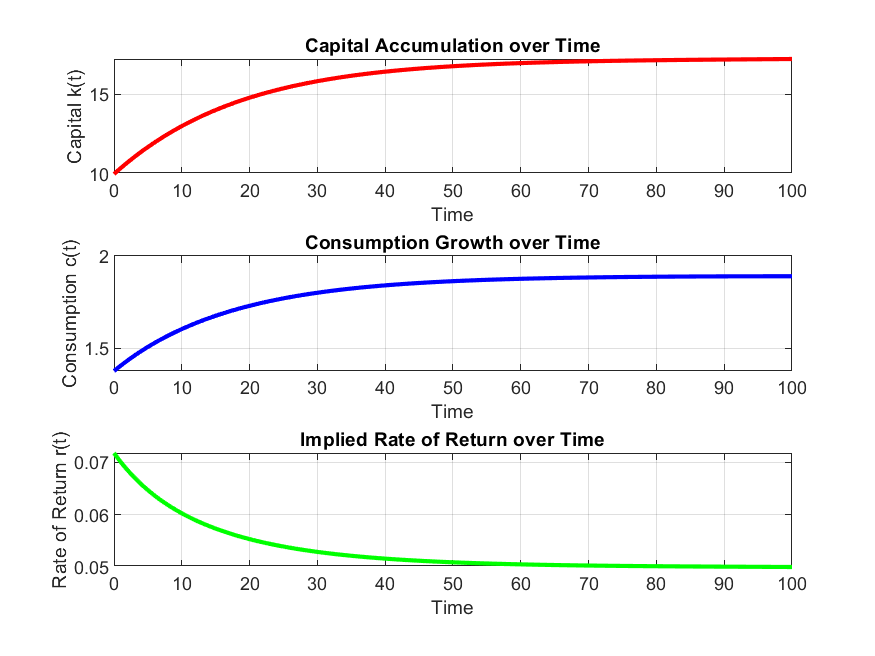
\includegraphics[width=\textwidth]{homework/Solutions/pset2.png}
\begin{lstlisting}
    % MATLAB code to solve for path of convergence using shooting method

clear all;
close all;
clc;

%% 1. DEFINE PARAMETERS
p = define_parameters();

%% 2. INITIALIZE GRID POINTS
t = linspace(p.tmin, p.tmax, p.I)';
dt = (p.tmax - p.tmin) / (p.I - 1);

%% 3. STEADY STATES
kss = ((p.rho + p.theta * p.g) / (p.alpha * p.A))^(1 / (p.alpha - 1));
css = p.f(kss) - (p.n + p.g) * kss;

%% 4. SHOOTING ALGORITHM

% Define objective function for initial consumption guess that matches terminal condition
diff = @(c0) terminal_condition(c0, p.k0, kss, p.f, p.f_prime, p.rho, p.theta, p.g, p.n, dt, p.I);

% Initial guess for consumption
c0_guess = 1;

% Solve for initial consumption using fsolve to satisfy k(T) = k_ss
options = optimoptions('fsolve', 'TolFun', p.tol, 'Display', 'iter');
c0 = fsolve(diff, c0_guess, options);

% Simulate with determined initial consumption
[k, c] = forward_simulate(c0, p.k0, p.f, p.f_prime, p.rho, p.theta, p.g, p.n, dt, p.I);

% 6.3 Calculate the implied rate of return r(t) = f'(k_t)
r_t = p.f_prime(k);

%% 7. PLOT

% 7-1. Evolution of capital, consumption, and rate of return

figure;
subplot(3,1,1);
plot(t, k, 'r-', 'LineWidth', 2);
xlabel('Time'); ylabel('Capital k(t)');
title('Capital Accumulation over Time');
grid on;

subplot(3,1,2);
plot(t, c, 'b-', 'LineWidth', 2);
xlabel('Time'); ylabel('Consumption c(t)');
title('Consumption Growth over Time');
grid on;

subplot(3,1,3);
plot(t, r_t, 'g-', 'LineWidth', 2);
xlabel('Time'); ylabel('Rate of Return r(t)');
title('Implied Rate of Return over Time');
grid on;

saveas(gcf, 'pset2.png');

%% Function Definitions

function p = define_parameters()
    % This function defines the model parameters.
    p.rho = 0.03;
    p.theta = 1;
    p.g = 0.02;
    p.n = 0.02;
    p.alpha = 1/3;
    p.A = 1;
    p.f = @(k) p.A * k.^p.alpha;
    p.f_prime = @(k) p.alpha * p.A * k.^(p.alpha - 1);
    p.k0 = 10;
    p.tmin = 0;
    p.tmax = 100;
    p.I = 300;
    p.tol = 1e-6;
end

function [k, c] = forward_simulate(c0, k0, f, f_prime, rho, theta, g, n, dt, I)
    % Solves the model's differential equations by forward simulation.
    k = zeros(I, 1);
    c = zeros(I, 1);
    k(1) = k0;
    c(1) = c0;
    for i = 1:I-1
        c(i+1) = c(i) + dt * (f_prime(k(i)) - rho - theta * g) / theta * c(i);
        k(i+1) = k(i) + dt * (f(k(i)) - c(i) - (n + g) * k(i));
    end
end

function difference = terminal_condition(c0, k0, kss, f, f_prime, rho, theta, g, n, dt, I)
    % Computes difference between terminal capital and steady-state.
    [k, ~] = forward_simulate(c0, k0, f, f_prime, rho, theta, g, n, dt, I);
    k_T = k(end);
    difference = k_T - kss;
end
\end{lstlisting}



\end{document}
